\begin{frame}{Neural Network considered}
    \vspace{-2pt}
    We consider a parametric NN with 4 inputs and 4 outputs, defined by
    $$U_\theta(\bm{x},\bm{\mu}) = \big(u_{1,\theta},u_{2,\theta},p_\theta,T_\theta)(\bm{x},\bm{\mu}).$$
    
    The Dirichlet boundary conditions are imposed on the outputs of the MLP by a \textbf{post-processing} step. \citep{Sukumar_2022}
    
    \begin{center}
        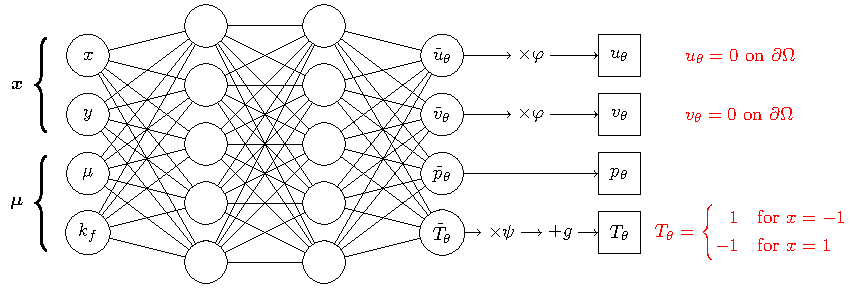
\includegraphics[width=0.85\linewidth]{images/pinn/network/network.pdf}
    \end{center}

    \vspace{-5pt}
    We consider two levelsets functions $\varphi_1$ and $\varphi_2$, and the linear function $g$ defined by
    \begin{equation*}
        \varphi_1(x,y) = (x-1)(x+1)(y-1)(y+1),
    \end{equation*}
    \begin{equation*}
        \varphi_2(x,y) = (x-1)(x+1) \quad \text{and} \quad g(x,y) = 1 - (x+1).
    \end{equation*}
\end{frame}

\begin{frame}{PINN training}
    \vspace{-4pt}
    \textbf{Approximate the solution of \eqref{eq:Pb} by a PINN :} Find the optimal weights $\theta^\star$, such that
	
    \vspace{-8pt}
    \begin{equation}
		\label{eq:opt_pb}
		\theta^\star = \argmin_{\theta}	\big( \; \textcolor{orange}{J_{inc}(\theta)} + \textcolor{orange}{J_{mom}(\theta)} + \textcolor{orange}{J_{ener}(\theta)} + \textcolor{darkred}{J_{ad}(\theta)} \; \big),
		\tag{$\mathcal{P}_\theta$}
	\end{equation}

    \vspace{-2pt}
	where the different cost functions\footnote[frame,1]{Discretized by a random process using Monte-Carlo method.} are defined by
	\vspace{5pt}

	\begin{minipage}{0.24\linewidth}
		\centering
		\textcolor{darkred}{adiabatic condition}
        
		\vspace{12pt}
		\textcolor{orange}{$3$ residual losses}
	\end{minipage}
	\begin{minipage}{0.68\linewidth}
		\centering
        \fcolorbox{darkred}{white}{
            $J_{ad}(\theta) =
            \int_{\mathcal{M}}\int_{\Gamma_\text{ad}} \big| \frac{\partial T_\theta(\bm{x},\bm{\mu})}{\partial n} \big|^2 d\bm{x} d\bm{\mu},$}
        
        \vspace{3pt}
		\fcolorbox{orange}{white}{
            $J_{\textbullet}(\theta) =
                \int_{\mathcal{M}}\int_{\Omega}
                \big| R_{\textbullet}(U_\theta(\bm{x},\bm{\mu});\bm{x},\bm{\mu}) \big|^2 d\bm{x} d\bm{\mu},$}
	\end{minipage}
    
    \vspace{5pt}
    with $U_\theta$ the parametric NN and $\textbullet$ the PDE considered (i.e. $inc$, $mom$ or $ener$).

    %\footnote[frame,2]{We consider a MLP with 5 hidden layers ($40,60,60,60,40$) and a 'sine' activation function. We train the PINN over $10000$ epochs ($3000$ ADAM / $7000$ LBFGS) with $40000$ collocation points in $\Omega$ and $30000$ points on the boundary $\partial\Omega\vert_{y=\pm 1}$.}
    
    \vspace{-7pt}
    \vspace{3pt}    
    \begin{center}
        \begin{minipage}{0.62\linewidth}
            \centering
            \vspace{-8pt}
            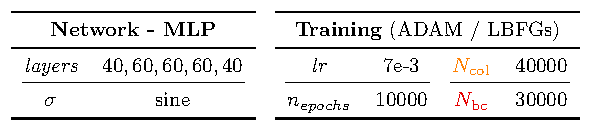
\includegraphics[width=0.94\linewidth]{images/pinn/training_param/training_param.pdf}
        \end{minipage}
        \begin{minipage}{0.36\linewidth}
            \centering
            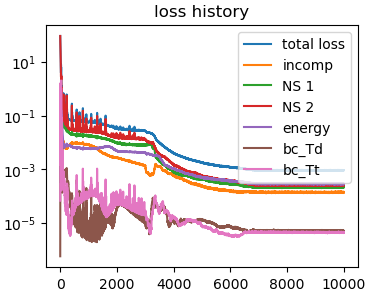
\includegraphics[width=0.84\linewidth]{images/pinn/training/test4_v5.png}
        \end{minipage}
    \end{center}
    
    \vspace{-8pt}
\end{frame}

\begin{frame}{Prediction on $\bm{\mu}^{(1)} = (0.1,0.1)$}
    \vspace{-4pt}
    \textbf{Prediction :} \begin{minipage}{0.26\linewidth}
        \centering
        $u_{1,\theta}$ \\
        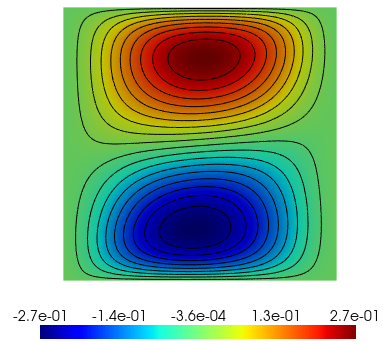
\includegraphics[width=0.95\linewidth]{images/pinn/training/PINN_plot_case4_v2_param1_u1.png}
    \end{minipage} \; \begin{minipage}{0.26\linewidth}
        \centering
        $u_{2,\theta}$ \\
        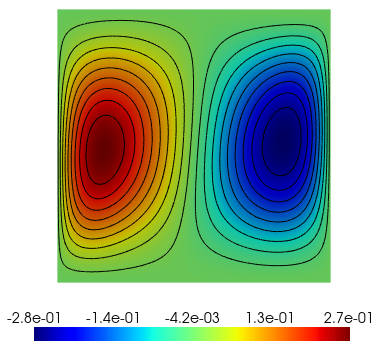
\includegraphics[width=0.95\linewidth]{images/pinn/training/PINN_plot_case4_v2_param1_u2.png}
    \end{minipage} \; \begin{minipage}{0.26\linewidth}
        \centering
        $T_\theta$ \\
        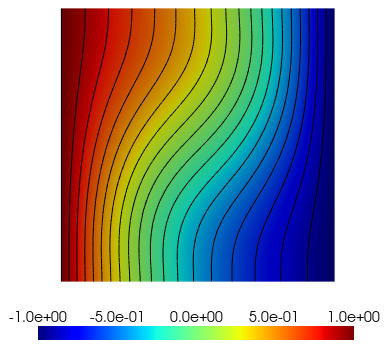
\includegraphics[width=0.95\linewidth]{images/pinn/training/PINN_plot_case4_v2_param1_T.png}
    \end{minipage}

    \vspace{8pt}

    \textbf{Error map :} \begin{minipage}{0.26\linewidth}
        \centering
        $u_{1,\text{ref}}-u_{1,\theta}$ \\
        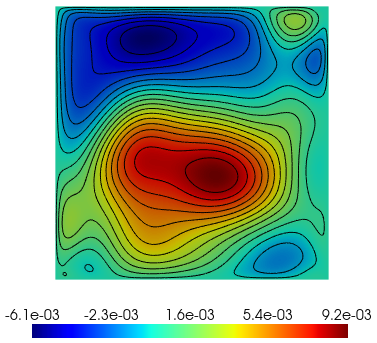
\includegraphics[width=0.95\linewidth]{images/pinn/training/PINN_error_plot_case4_v2_param1_u1.png}
    \end{minipage} \; \begin{minipage}{0.26\linewidth}
        \centering
        $u_{2,\text{ref}}-u_{2,\theta}$ \\
        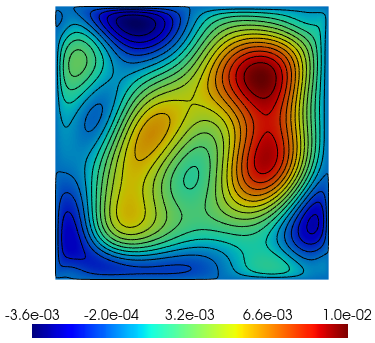
\includegraphics[width=0.95\linewidth]{images/pinn/training/PINN_error_plot_case4_v2_param1_u2.png}
    \end{minipage} \; \begin{minipage}{0.26\linewidth}
        \centering
        $T_\text{ref}-T_\theta$ \\
        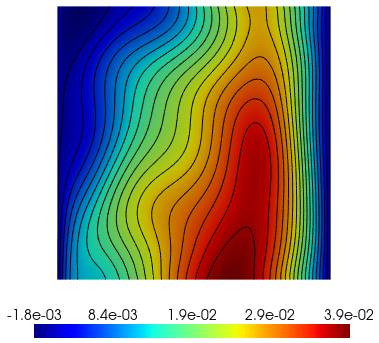
\includegraphics[width=0.95\linewidth]{images/pinn/training/PINN_error_plot_case4_v2_param1_T.png}
    \end{minipage}

    \vspace{8pt}

    \textbf{$L^2$ error :} \hspace{25pt} $2.98\times10^{-2} \hspace{42pt} 3.17\times10^{-2} \hspace{42pt}  3.90\times10^{-2}$

\end{frame}